% !TEX program = pdflatex
% Overleaf: main.tex, pdfLaTeX, BibTeX. No shell escape or custom fonts.
\documentclass[10pt,twocolumn]{article}
\usepackage[letterpaper,margin=0.72in,columnsep=0.25in]{geometry}
\usepackage[T1]{fontenc}
\usepackage{iftex}
\ifPDFTeX\usepackage[utf8]{inputenc}\fi
\usepackage{lmodern,microtype}
\usepackage{amsmath,amssymb}
\usepackage{graphicx,booktabs,tabularx,array,multirow,xcolor}
\usepackage{enumitem,listings}
\usepackage[numbers,sort&compress]{natbib}
\usepackage[font=small,labelfont=bf]{caption}
\usepackage{placeins,balance,url,hyperref}
\hypersetup{colorlinks=true,linkcolor=blue!45!black,citecolor=blue!45!black,urlcolor=blue!45!black,
pdftitle={Chinese Decision: A Family of Language Models for Single-Pass Probabilistic Decision-Making},pdfauthor={yanqiang}}
\setlength{\emergencystretch}{1.5em}
\setlist[itemize]{leftmargin=*,nosep,topsep=3pt}
\setlist[enumerate]{leftmargin=*,nosep,topsep=3pt}
\setlength{\textfloatsep}{12pt plus 2pt minus 2pt}
\raggedbottom
\setcounter{dbltopnumber}{3}
\renewcommand{\dbltopfraction}{0.88}
\renewcommand{\textfraction}{0.08}
\newcommand{\model}{\textsc{Chinese Decision}}
\newcommand{\noul}{\texttt{noul}}
\newcommand{\choice}{\texttt{choice}}
\newcommand{\score}{\texttt{score}}
\newcommand{\CE}{\mathcal{L}_{\mathrm{CE}}}
\newcommand{\R}{\mathbb{R}}
\newcommand{\ind}{\mathbf{1}}
\newcommand{\best}[1]{\textbf{#1}}
\lstset{basicstyle=\ttfamily\scriptsize,breaklines=true,columns=fullflexible,keepspaces=true,frame=single,
rulecolor=\color{black!18},backgroundcolor=\color{black!2},showstringspaces=false,xleftmargin=3pt,xrightmargin=3pt}
\title{\textbf{Chinese Decision: A Family of Language Models for\\Single-Pass Probabilistic Decision-Making}}
\author{yanqiang\\Institute of Computing Technology, Chinese Academy of Sciences\\\texttt{yanqiang@ict.ac.cn}}
\date{Technical Report --- October 16, 2026}
\begin{document}
\maketitle
\begin{abstract}
Many language-based applications require a probability distribution over a small set of decisions rather than an open-ended response. We present \model, a family of Chinese-language decision models that adapts pretrained causal language models to this interface. Each question is compiled into a shared instruction-and-candidate prompt; a single forward pass extracts the final-position logits of candidate letters and normalizes them over the valid options, without autoregressive answer generation. The interface covers Boolean judgments, categorical choices, and ordinal scores. We report a completed 0.8B model trained with distribution cross-entropy on 13.048 million decisions, together with preliminary 2B checkpoints trained with an additional RLCD objective. On the full 307,900-decision CJ-Bench, the uncalibrated 0.8B model achieves 72.24\% general-domain accuracy and 76.98\% average accuracy across medicine, law, and finance using one shared checkpoint. Its overall expected calibration error is 1.07\%. The 2B model reaches 72.56\% general-domain accuracy after 40.13\% of one training epoch, but has not yet surpassed the completed 0.8B model on the professional-domain average. We also evaluate a validation-temperature-scaled deployment model and its Q8 quantization, documenting both aggregate preservation and individual prediction changes. These results establish a reproducible training and deployment path for Chinese probabilistic decisions; they do not isolate the causal effect of model scale.
\end{abstract}
\section{Introduction}
\label{sec:intro}
A customer-support system may need to select a department, a moderation service to decide whether to escalate a message, and an agent to choose an available tool. In each case, the output space is bounded, even though the input and the decision instructions are expressed in natural language. A generative interface can encode these tasks, but applications must then recover a decision from generated text. When downstream logic depends on uncertainty, a label alone is also insufficient: the application needs probabilities over the alternatives.

\model{} exposes this bounded decision problem directly. It accepts a context, a question, and candidate descriptions, and returns a normalized probability distribution. The same distribution supports a Boolean judgment, a categorical selection, or the expected value of an ordered rating. The model processes each question once and reads existing vocabulary logits at the final input position. No answer token is sampled, no free-form answer is parsed, and no chain of thought is generated. Here, \emph{single-pass} refers to one forward evaluation per compiled question; it does not imply constant work independent of input length or that all questions in an API request share one forward evaluation.

The project builds on the option-letter decision workflow in \texttt{hmm}~\citep{hmm2026}, Qwen3.5 language backbones~\citep{qwen08,qwen2b}, and the CJ-Dataset and CJ-Bench resources~\citep{wang2026chinesejev}. Our focus is adaptation, joint-domain training, empirical characterization, and deployment of a reusable Chinese decision model. We do not introduce the candidate-letter readout, underlying language architecture, or upstream benchmark as new methods.

The initial completed member uses the Qwen3.5-0.8B text backbone and low-rank adaptation~\citep{hu2021lora}. It is trained for one epoch on all four CJ domains using probability-distribution targets. One checkpoint serves the general, medical, legal, and financial subsets. The next member uses Qwen3.5-2B; its currently available checkpoints additionally use RLCD and a larger training batch. We report those snapshots explicitly as preliminary rather than presenting an unfinished model as a completed release.

This distinction matters empirically. The completed 0.8B model achieves 72.24\% general accuracy and 76.98\% professional-domain average accuracy. The 2B step-2000 snapshot reaches 72.56\% general accuracy but 74.22\% on the professional average. The evidence supports a useful common interface across model sizes, while leaving a controlled analysis of scaling to future experiments.

Our contributions are threefold:
\begin{itemize}
\item A shared Chinese decision pipeline for Boolean, categorical, and ordinal questions, including distribution supervision, train/evaluation/serving prompt consistency, and separate validation partitions for selection and temperature fitting.
\item A full CJ-Bench study of the completed 0.8B member, checkpoint trajectories, and preliminary 2B members, with explicit separation of imported baselines, local measurements, and experimental confounders.
\item An open deployment implementation with Transformers and GGUF backends, accompanied by full-benchmark quantization comparisons and scoped CPU and GPU measurements.
\end{itemize}

Code, released 0.8B weights, and the application workbench are available online.\footnote{\href{https://github.com/yanqiangmiffy/chinese-decision}{Source code}; \href{https://huggingface.co/quincyqiang/chinese-decision-0.8b}{0.8B model}; \href{https://github.com/yanqiangmiffy/chinese-decision-studio}{Decision Studio}.}

\section{Related Work}
\label{sec:related}
\paragraph{Bounded decisions with language models.}
Candidate descriptions allow one model to express multiple classification tasks without a separate application-specific output vocabulary. The \texttt{hmm} implementation~\citep{hmm2026} uses answer-letter logits and LoRA for structured decision prediction. We adapt that design to Chinese prompts and distribution-valued supervision. The readout is a constrained classification distribution derived from a language-model head, rather than a distribution over generated answer strings.

\paragraph{Chinese decision resources.}
Chinese-Jev~\citep{wang2026chinesejev} provides the data and benchmark used here, and studies an encoder-based decision system with general training followed by specialist adaptation. Our implementation instead jointly adapts a causal language backbone across domains. Differences in backbone, objective, and training allocation prevent attributing performance gaps to a single architectural choice.

\paragraph{Adaptation and calibration.}
LoRA~\citep{hu2021lora} restricts parameter updates to low-rank matrices that can be merged into the backbone. Temperature scaling~\citep{guo2017calibration} adjusts predictive sharpness using a scalar fitted on held-out data. We use these established techniques and distinguish the raw checkpoint from the temperature-scaled deployment artifact. A low aggregate calibration error is an empirical property of a specified evaluation distribution, not a guarantee for arbitrary application inputs.

\section{Method}
\label{sec:method}
\subsection{Decision Representation}
A decision example consists of a context $s$, an instruction $u$, an ordered list of candidates $\mathcal{C}=\{(k_i,d_i)\}_{i=1}^{K}$, and a target probability vector $\mathbf{y}\in\Delta^{K-1}$. Here $k_i$ is an application-facing key, $d_i$ its natural-language description, and $2\leq K\leq26$. Hard labels are one-hot vectors; soft labels retain the upstream distribution. Input validation requires finite, nonnegative targets with total mass one up to a numerical tolerance.

The interface has three question types. \noul{} is a proposition judgment with candidates ordered as false and true; its scalar result is $p(\mathrm{true})$. \choice{} returns the key with the largest probability. \score{} takes rating levels in increasing order and returns
\begin{equation}
\hat r=\sum_{i=1}^{K}(i-1)p_i.
\label{eq:score}
\end{equation}
The full distribution is retained in all cases. This expectation treats adjacent level indices as equally spaced; it does not establish equal semantic distance between arbitrary rating descriptions.

\subsection{Shared Prompt Compilation}
The compiler associates candidates with the letters A through Z, renders the context, question, candidate keys and descriptions, and applies the backbone's chat template with thinking disabled. Training, benchmarking, and serving call the same compiler, identified as \texttt{hmm-zh-v1}. Appendix~\ref{app:prompt} gives an English translation of its Chinese user-message body.

The implementation accepts at most 16,384 input tokens. Training explicitly counts and filters overlength examples; evaluation fails on overflow and serving rejects overlength requests. The full benchmark runs reported here have zero filtered or truncated decisions. This implementation limit is distinct from the backbone's native context capacity.

\begin{figure*}[t]
\centering
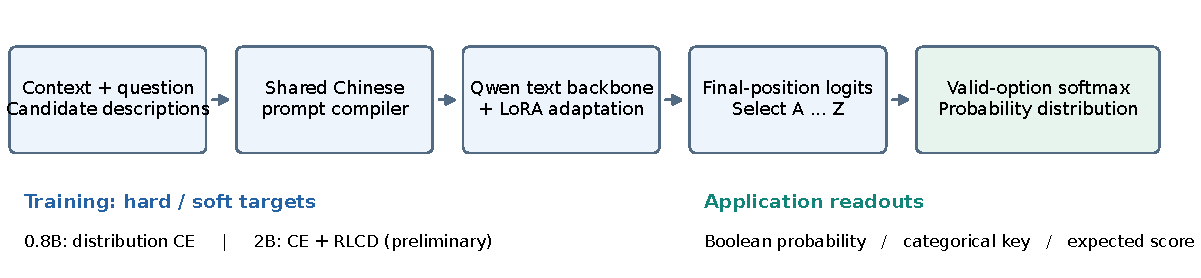
\includegraphics[width=\textwidth]{figures/pipeline.pdf}
\caption{The shared decision path. Each compiled question is evaluated once. Candidate-letter logits are normalized only over valid candidates. Training supplies hard or soft target distributions; deployment maps the same probabilities to a Boolean result, a categorical key, or an expected ordinal score. Multiple questions can be batched, but remain distinct compiled inputs.}
\label{fig:pipeline}
\end{figure*}

\subsection{Single-Pass Candidate Probabilities}
Let $x=\phi(s,u,\mathcal{C})$ be the tokenized prompt of length $L$. A causal language model produces vocabulary logits $\mathbf{v}_{L}\in\R^{|V|}$ at the final position. If $t_i$ is the token ID for candidate letter $i$, we select $z_i=v_{L,t_i}$ and compute
\begin{equation}
p_i(\mathbf{z};T)=\frac{\exp(z_i/T)}{\sum_{j=1}^{K}\exp(z_j/T)},\qquad T>0.
\label{eq:softmax}
\end{equation}
The tokenizer is checked to ensure that every candidate letter is a single token. Invalid letters are masked before normalization. The output is conditioned on the provided candidate set and excludes vocabulary mass assigned to other tokens. These are decision probabilities learned under candidate supervision, rather than unrestricted next-token probabilities or probabilities of open-ended answer correctness.

Only final-position language-model logits are requested from the backbone. The input sequence still passes through its full text network. The method removes iterative answer generation; it does not remove prompt processing or guarantee lower latency than a compact encoder.

\subsection{Distribution Supervision and LoRA}
The completed 0.8B member minimizes distribution cross-entropy:
\begin{equation}
\CE(\theta)=-\frac{1}{N}\sum_{n=1}^{N}\sum_{i=1}^{K_n}y_{ni}\log p_{\theta,i}(x_n;1).
\label{eq:ce}
\end{equation}
Because $\mathbf{y}$ may be soft, this objective retains information discarded by replacing every target with its argmax. For fixed targets it differs from $D_{\mathrm{KL}}(\mathbf{y}\Vert\mathbf{p})$ only by target entropy. It does not explicitly penalize ordinal distance between rating levels.

For a frozen backbone matrix $W_0$, LoRA learns $W=W_0+(\alpha/r)BA$. Both reported model sizes use rank $r=32$, $\alpha=64$, and dropout 0.05. Adapters target full-attention, linear-attention, and feed-forward projections. The released 0.8B weights merge the selected adapter into the backbone; Appendix~\ref{app:reproduce} lists the target modules.

During training, \choice{} candidates and their target probabilities are jointly permuted. \noul{} retains false/true order and \score{} retains level order. Permutation augmentation is intended to reduce dependence on categorical candidate position, but the experiments below do not measure permutation invariance directly.

\subsection{RLCD in the Preliminary 2B Run}
\label{sec:rlcd}
The 2B run adds an RLCD term adapted from the upstream implementation. For logits $\mathbf{z}$, it samples $M=4$ Gaussian perturbations, centers each perturbation over valid candidates, and forms
\begin{equation}
\mathbf{z}^{(m)}=\operatorname{sg}(\mathbf{z})+\tilde{\boldsymbol\epsilon}^{(m)},
\quad \mathbf{q}^{(m)}=\operatorname{softmax}(\mathbf{z}^{(m)}),
\end{equation}
where $\operatorname{sg}$ stops gradients. The reward combines a clipped log score, a spherical score, and a ranked probability score for ordinal questions:
\begin{align}
R(\mathbf{q},\mathbf{y})={}&\sum_i y_i\max(\log q_i,-9.21)\nonumber\\
&+0.75\frac{\mathbf{y}^{\top}\mathbf{q}}{\|\mathbf{q}\|_2}
-\ind_{\score}\operatorname{RPS}(\mathbf{q},\mathbf{y}),\label{eq:reward}\\
\operatorname{RPS}(\mathbf{q},\mathbf{y})={}&\frac{1}{K-1}\sum_{k=1}^{K}
\left(\sum_{i=1}^{k}(q_i-y_i)\right)^2.\label{eq:rps}
\end{align}
The final cumulative term is zero for normalized distributions. The implementation uses small numerical floors in logarithms and norms. Because the logarithmic reward is clipped, we make no blanket claim that the implemented composite reward is strictly proper over the entire probability simplex.

Let $A_m$ be the reward after subtracting the per-example perturbation-group mean. Advantages are divided by their standard deviation over the perturbation-by-microbatch tensor plus $10^{-6}$ and detached. The surrogate is
\begin{align}
\mathcal{L}_{\mathrm{RLCD}}&=-\frac1M\sum_m\operatorname{sg}(A_m)\ell_m(\mathbf{z}),\\
\ell_m(\mathbf{z})&=-\frac{\|\mathbf{z}^{(m)}-\mathbf{z}\|_2^2}{2\sigma^2},\label{eq:rlcd}
\end{align}
with an additional average over examples. The 2B objective is $\CE+\mathcal{L}_{\mathrm{RLCD}}$, with unit weights. The noise scale decreases linearly from 0.4 to 0.1 with the fraction of the planned epoch consumed. All completed 0.8B results use cross-entropy alone. Thus 0.8B--2B comparisons change both size and objective.

\subsection{Held-Out Temperature and Output Semantics}
\label{sec:temperature}
The official validation split is partitioned by a deterministic hash of parent-record identity. Four of five hash buckets are eligible for model selection; the remaining bucket is reserved for temperature fitting. Reservoir sampling selects up to 100 decisions per domain/type stratum for selection, yielding 1,200 examples. Checkpoints are chosen by distribution negative log-likelihood (NLL), not test accuracy or ECE.

For the 0.8B release, a scalar temperature is fitted on hard labels sampled from the reserved bucket by minimizing cross-entropy. This produces $T=1.108133$ from 1,993 hard-labeled calibration decisions. No test labels are used for fitting. We report $T=1$ for main checkpoint comparisons and use the fixed fitted temperature only in the deployment study.

The API also returns a normalized sharpness statistic
\begin{equation}
c=\frac{K\max_i p_i-1}{K-1}.\label{eq:confidence}
\end{equation}
It is zero for a uniform distribution and one for a point mass. It is not an empirical correctness probability. Benchmark ECE uses $\max_i p_i$, not $c$.

\section{Experimental Setup}
\label{sec:setup}
\subsection{Data and Mixing}
We use the released CJ training and benchmark splits rather than constructing a new corpus. The training split contains 13,048,000 decisions: 10,000,000 general, 3,000,000 medical, and 24,000 each in law and finance. Table~\ref{tab:data} reports split sizes and hard-label counts used in evaluation. Counts refer to decisions, not unique source documents or independent real-world events.

\begin{table}[t]
\centering
\footnotesize
\setlength{\tabcolsep}{4pt}
\caption{Training and full CJ-Bench sizes. Accuracy and ECE use only hard test targets.}
\label{tab:data}
\begin{tabular}{lrrr}
\toprule
Domain & Train & Test & Hard test \\
\midrule
General & 10,000,000 & 100,000 & 96,922 \\
Medical & 3,000,000 & 200,000 & 200,000 \\
Legal & 24,000 & 4,300 & 4,300 \\
Finance & 24,000 & 3,600 & 3,600 \\
Total & 13,048,000 & 307,900 & 304,822 \\
\bottomrule
\end{tabular}
\end{table}


Training data are sharded by domain, source, and question type. A streaming mixer samples shards in proportion to their remaining counts and visits each decision once per epoch. This interleaves tasks while retaining corpus proportions; it does \emph{not} equalize domain frequencies or oversample the smaller domains. Length bucketing and padded-token budgets reduce padding overhead. Validation files are not mixed into training.

A separate full-file candidate-count audit checks release checksums and finds 2--16 candidates in the training, validation, and test splits, with no decision exceeding 26 candidates. Thus the 26-letter interface does not exclude released benchmark decisions. This audit verifies format and coverage, not freedom from pretraining contamination.

\subsection{Training Configurations}
\begin{table}[t]
\centering
\footnotesize
\setlength{\tabcolsep}{4pt}
\caption{Recorded training configurations. The 2B run is ongoing at the evidence snapshot.}
\label{tab:training}
\begin{tabular}{p{0.40\columnwidth}rr}
\toprule
Setting & 0.8B & 2B \\
\midrule
Objective & CE & CE + RLCD \\
LoRA rank / scaling & 32 / 64 & 32 / 64 \\
Dropout & 0.05 & 0.05 \\
Peak learning rate & $10^{-4}$ & $10^{-4}$ \\
Nominal minimum batch & 1,024 & 2,048 \\
Global token budget & 262,144 & 524,288 \\
Bucketing pool & 4,096 & 4,096 \\
Maximum input & 16,384 & 16,384 \\
Planned epochs & 1 & 1 \\
Reported latest step & 10,000 & 2,000 \\
Final optimizer step & 10,132 & Ongoing \\
RLCD perturbations & -- & 4 \\
RLCD $\sigma$ schedule & -- & $0.4\to0.1$ \\
Random seed & 42 & 42 \\
\bottomrule
\end{tabular}
\par\vspace{3pt}\begin{minipage}{\columnwidth}\footnotesize Token budgets are padded-token limits shared across ranks. Accumulation can exceed the nominal minimum batch.\end{minipage}
\end{table}

Table~\ref{tab:training} gives the run configurations. The 0.8B run completes one epoch in 10,132 optimizer updates; its minimum validation NLL occurs at step 10,000. Training uses BF16, gradient checkpointing, AdamW, peak learning rate $10^{-4}$, gradient norm clipping at 1.0, 100-step warmup, and cosine decay toward 10\% of peak. The effective schedule multiplies the warmup factor by the cosine factor.

The nominal global batch is a minimum decision count accumulated before an update, rather than a fixed exact size. Token-limited microbatches can overshoot this threshold; gradients are normalized by the actual decision count. Optimizer steps therefore do not provide matched data exposure across sizes. The 2B step-1000 and step-2000 snapshots have consumed 2,619,904 and 5,236,736 decisions (20.08\% and 40.13\% of one epoch). They are validation-selected snapshots available during an ongoing one-epoch run.

The completed 0.8B run uses four GPUs in its final configuration, following an earlier change in distributed world size recorded by the project. We lack consolidated energy or GPU-hour accounting and make no training-cost-efficiency claim.

\subsection{Metrics and Evaluation Protocol}
Every full run covers all 307,900 CJ-Bench decisions, including 304,822 hard targets and 3,078 soft targets. Candidate order is preserved during testing. Inputs are neither filtered nor truncated; the longest compiled prompt is 6,850 tokens and the mean length is 222.53 tokens.

Accuracy uses argmax predictions on hard targets only. ECE uses the same hard subset and 15 equal-width confidence bins:
\begin{equation}
\mathrm{ECE}=\sum_{b=1}^{15}\frac{|B_b|}{N_h}
\left|\mathrm{acc}(B_b)-\mathrm{conf}(B_b)\right|,\label{eq:ece}
\end{equation}
where confidence is the maximum candidate probability. Distribution NLL and the unnormalized multiclass Brier score use all targets:
\begin{align}
\mathrm{NLL}&=-\frac{1}{N}\sum_{n,i}y_{ni}\log p_{ni},\\
\mathrm{Brier}&=\frac{1}{N}\sum_{n,i}(p_{ni}-y_{ni})^2.
\end{align}
For \score{}, expected-score MAE compares expected level indices under the predicted and target distributions. Ordinal accuracy still uses discrete argmax and is a different metric.

We report micro accuracy over all hard targets, four-domain macro accuracy, and the unweighted average across three professional domains. Medicine accounts for 64.96\% of all decisions and 65.61\% of hard targets, so micro and macro performance answer different questions. Training-time validation summaries use 10 ECE bins; they are not directly interchangeable with 15-bin benchmark ECE. Model selection always uses distribution NLL.

\subsection{Baselines and Evidence Provenance}
Baseline accuracies and ECE values are imported from Tables 1 and 2 of Chinese-Jev~\citep{wang2026chinesejev}; we do not rerun those models. Chinese-Jev-G denotes its general checkpoint and Chinese-Jev-S denotes three domain specialists. Jev is a hosted model. The imported Qwen3.5-2B baseline is not our decision-fine-tuned 2B model.

Local tables are generated from stored evaluation JSON files, with source paths and SHA256 hashes recorded in the accompanying artifact. The manuscript uses an October 16, 2026 evidence snapshot. We have not repeated GPU training or inference during manuscript preparation. Imported baseline latency is omitted from the accuracy tables because hardware and, for Jev, network scope differ from our measurements.

\section{Results and Analysis}
\label{sec:results}
\subsection{General and Professional Decisions}
\begin{table}[t]
\centering
\footnotesize
\setlength{\tabcolsep}{4pt}
\caption{General-domain comparison. All local models use $T=1$; 2B results are preliminary.}
\label{tab:general}
\begin{tabular}{lrr}
\toprule
Model & ACC (\%) $\uparrow$ & ECE (\%) $\downarrow$ \\
\midrule
Qwen3.5-2B (imported) & 32.95 & 43.68 \\
Open-Jev & 52.33 & 10.54 \\
SemIF & 44.21 & 27.27 \\
Laya Multilingual & 40.22 & 23.04 \\
Jev & 68.35 & 11.45 \\
Chinese-Jev General & 69.20 & 3.78 \\
Ours 0.8B (step 10000) & 72.24 & 3.03 \\
Ours 2B (step 1000) & 70.55 & 4.58 \\
Ours 2B (step 2000) & 72.56 & 2.93 \\
\bottomrule
\end{tabular}
\par\vspace{3pt}\begin{minipage}{\columnwidth}\footnotesize Baseline rows are imported from Chinese-Jev~\citep{wang2026chinesejev}, not reproduced. The decision-fine-tuned 2B members differ from the imported Qwen baseline.\end{minipage}
\end{table}

Table~\ref{tab:general} compares general-domain performance. The completed 0.8B member reaches 72.24\% accuracy, 3.04 percentage points above the imported Chinese-Jev General result and 3.89 points above Jev. Its ECE is 3.03\%, compared with 3.78\% and 11.45\%, respectively. The preliminary 2B step-2000 checkpoint reaches 72.56\% accuracy and 2.93\% ECE. These comparisons describe the reported benchmark results; confidence intervals and a locally rerun baseline comparison are not available.

\begin{table*}[t]
\centering
\small
\setlength{\tabcolsep}{4pt}
\caption{Professional-domain comparison: accuracy / ECE (\%). Each local row uses one checkpoint for all domains; 2B snapshots are preliminary and uncalibrated.}
\label{tab:professional}
\begin{tabular}{lrrrrrrrr}
\toprule
& \multicolumn{2}{c}{Medical} & \multicolumn{2}{c}{Legal} & \multicolumn{2}{c}{Finance} & \multicolumn{2}{c}{Professional mean} \\ Model & ACC $\uparrow$ & ECE $\downarrow$ & ACC $\uparrow$ & ECE $\downarrow$ & ACC $\uparrow$ & ECE $\downarrow$ & ACC $\uparrow$ & ECE $\downarrow$ \\
\midrule
Qwen3.5-2B (imported) & 53.88 & 28.71 & 31.53 & 44.82 & 38.11 & 49.12 & 41.17 & 40.88 \\
Open-Jev & 73.08 & 2.88 & 44.07 & 23.15 & 48.11 & 10.19 & 55.09 & 12.07 \\
SemIF & 62.17 & 10.39 & 43.07 & 19.99 & 47.89 & 18.45 & 51.04 & 16.28 \\
Laya Multilingual & 24.55 & 43.05 & 34.72 & 31.49 & 38.31 & 26.18 & 32.53 & 33.57 \\
Jev & 84.29 & 5.70 & 68.35 & 8.03 & 78.39 & 2.98 & 77.01 & 5.57 \\
Chinese-Jev-S (3 models) & 87.65 & 7.25 & 60.10 & 17.45 & 64.72 & 11.55 & 70.82 & 12.08 \\
Ours 0.8B (single model) & 88.86 & 0.17 & 67.86 & 5.70 & 74.22 & 1.50 & 76.98 & 2.46 \\
Ours 2B (step 1000) & 87.69 & 0.67 & 55.67 & 6.83 & 66.94 & 3.63 & 70.10 & 3.71 \\
Ours 2B (step 2000) & 88.54 & 0.41 & 62.67 & 4.11 & 71.44 & 2.32 & 74.22 & 2.28 \\
\bottomrule
\end{tabular}
\par\vspace{3pt}\begin{minipage}{\textwidth}\footnotesize All baseline values are imported from Chinese-Jev~\citep{wang2026chinesejev}. The last baseline combines three specialist models. Means are unweighted across the three domains.\end{minipage}
\end{table*}

One 0.8B checkpoint covers all professional domains in Table~\ref{tab:professional}. It obtains 88.86\% medical, 67.86\% legal, and 74.22\% financial accuracy. Each exceeds the corresponding imported Chinese-Jev specialist result, by 1.21, 7.76, and 9.50 points. Its 76.98\% professional average is numerically close to Jev's 77.01\%, but this 0.03-point difference is not evidence of statistical equivalence. The model exceeds Jev in medicine, trails it by 0.49 points in law, and trails it by 4.17 points in finance.

The professional-domain average ECE is 2.46\% for 0.8B and 2.28\% for the 2B step-2000 snapshot. In the latter case, lower average ECE coexists with lower average accuracy (74.22\%). Accuracy and calibration therefore need to be examined jointly; neither is a substitute for the other.

\subsection{Aggregate and Typed Results}
\begin{table*}[t]
\centering
\small
\setlength{\tabcolsep}{4pt}
\caption{Full-benchmark aggregate results at $T=1$. Macro ACC averages four domains; score MAE is restricted to ordinal questions.}
\label{tab:aggregate}
\begin{tabular}{lrrrrrr}
\toprule
Model / checkpoint & Micro ACC (\%) & Macro ACC (\%) & ECE (\%) & NLL & Brier & Score MAE \\
\midrule
0.8B / step 10000 & 83.11 & 75.80 & 1.07 & 0.432 & 0.224 & 0.579 \\
2B / step 1000 & 81.55 & 70.22 & 2.03 & 0.493 & 0.248 & 0.612 \\
2B / step 2000 & 82.89 & 73.80 & 1.27 & 0.447 & 0.228 & 0.583 \\
\bottomrule
\end{tabular}
\end{table*}

Table~\ref{tab:aggregate} reports complementary aggregate metrics. The completed 0.8B model obtains 83.11\% micro accuracy and 75.80\% four-domain macro accuracy. The gap reflects the weight of the larger and easier medical subset. The 2B step-2000 snapshot obtains 82.89\% micro and 73.80\% macro accuracy, with distribution NLL 0.447 versus 0.432 for 0.8B.

\begin{table*}[t]
\centering
\small
\setlength{\tabcolsep}{4pt}
\caption{Question-type results at $T=1$. The 2B row group is preliminary. The total/hard counts identify the metric denominators.}
\label{tab:types}
\begin{tabular}{llrrrrr}
\toprule
Model / step & Type & Total / hard & ACC (\%) & ECE (\%) & NLL & Score MAE \\
\midrule
0.8B / 10000 & \texttt{noul} & 134,577 / 134,577 & 94.95 & 0.39 & 0.117 & -- \\
0.8B / 10000 & \texttt{choice} & 134,577 / 134,577 & 78.33 & 1.48 & 0.588 & -- \\
0.8B / 10000 & \texttt{score} & 38,746 / 35,668 & 56.47 & 2.35 & 0.987 & 0.579 \\
2B / 2000 & \texttt{noul} & 134,577 / 134,577 & 94.77 & 1.04 & 0.124 & -- \\
2B / 2000 & \texttt{choice} & 134,577 / 134,577 & 78.36 & 1.06 & 0.604 & -- \\
2B / 2000 & \texttt{score} & 38,746 / 35,668 & 55.18 & 3.04 & 1.024 & 0.583 \\
\bottomrule
\end{tabular}
\end{table*}

Question-type results in Table~\ref{tab:types} show that Boolean judgments are substantially easier than categorical and ordinal decisions in this benchmark. The 0.8B model reaches 94.95\% \noul{} accuracy, 78.33\% \choice{} accuracy, and 56.47\% hard-target \score{} accuracy. Its expected-score MAE is 0.579 level indices. The larger run is slightly higher on categorical accuracy at step 2000 (78.36\%), but lower on Boolean and ordinal accuracy. Because candidate counts, source tasks, and domain mixtures differ by type, these gaps should not be interpreted as controlled effects of interface design alone.

\subsection{Training Trajectories}
\begin{table*}[t]
\centering
\footnotesize
\setlength{\tabcolsep}{4pt}
\caption{Checkpoint trajectory for the 0.8B cross-entropy run. All test results are full-benchmark, uncalibrated measurements.}
\label{tab:trajectory}
\begin{tabular}{rrrrrrrrr}
\toprule
Step & Val. NLL & General ACC & Medical ACC & Legal ACC & Finance ACC & Prof. ACC & Prof. ECE & Micro ECE \\
\midrule
2,000 & 0.739 & 69.04 & 86.78 & 54.07 & 64.17 & 68.34 & 2.73 & 1.63 \\
3,000 & 0.691 & 70.26 & 87.22 & 58.93 & 68.67 & 71.61 & 1.75 & 1.25 \\
5,000 & 0.676 & 70.90 & 87.89 & 63.37 & 71.17 & 74.14 & 1.49 & 0.84 \\
10,000 & 0.600 & 72.24 & 88.86 & 67.86 & 74.22 & 76.98 & 2.46 & 1.07 \\
\bottomrule
\end{tabular}
\par\vspace{3pt}\begin{minipage}{\textwidth}\footnotesize Accuracy and ECE are percentages. Checkpoints are selected using validation distribution NLL, not these test metrics.\end{minipage}
\end{table*}

\begin{figure*}[t]
\centering
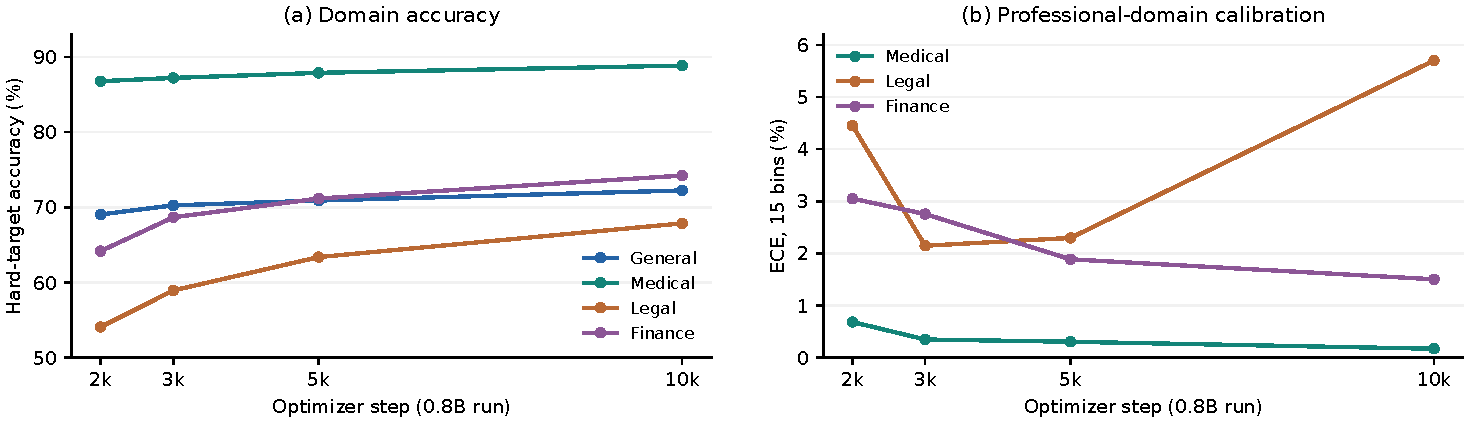
\includegraphics[width=\textwidth]{figures/trajectory.pdf}
\caption{Checkpoints from the same 0.8B cross-entropy run. Left: accuracy improves across all four domains. Right: professional-domain ECE does not improve monotonically; the legal subset worsens late in training. All points use full CJ-Bench evaluation at $T=1$. Lines connect measured checkpoints and do not represent independent training replicates.}
\label{fig:trajectory}
\end{figure*}
Across the four validation-selected 0.8B checkpoints in Table~\ref{tab:trajectory} and Figure~\ref{fig:trajectory}, validation distribution NLL falls from 0.739 to 0.600. Legal accuracy rises from 54.07\% to 67.86\%, finance from 64.17\% to 74.22\%, general from 69.04\% to 72.24\%, and medicine from 86.78\% to 88.86\%. The strongest gains are in the two domains with the least training data, although this observation alone does not establish the mechanism of transfer.

Calibration is non-monotonic. The professional average ECE is 2.73\%, 1.75\%, 1.49\%, and 2.46\% at steps 2000, 3000, 5000, and 10000. Legal ECE rises from 2.30\% at step 5000 to 5.70\% at step 10000 even as legal accuracy improves. Choosing the checkpoint with the best test ECE would conflict with the stated selection protocol; the released checkpoint remains the one selected by validation NLL.

\subsection{What the 2B Snapshots Establish}
The 2B run improves across both available full evaluations. Between steps 1000 and 2000, general accuracy rises from 70.55\% to 72.56\%, medicine from 87.69\% to 88.54\%, law from 55.67\% to 62.67\%, and finance from 66.94\% to 71.44\%. The professional average rises from 70.10\% to 74.22\%, and micro ECE falls from 2.03\% to 1.27\%.

At 40.13\% of the planned epoch, 2B has a higher general-domain point estimate than the completed 0.8B run by 0.31 points, but is lower in the other three domains. Neither completion quality nor monotonic gains with scale can be inferred. Size, training objective, minimum batch, token budget, and consumed data all differ. In particular, there is no matched 2B cross-entropy-only run here that would isolate RLCD, and no completed 2B result that would isolate training completion. We use ``family'' to denote a common model interface and adaptation pipeline across the two instantiated sizes, not a demonstrated scaling law.

\section{Deployment and Quantization}
\label{sec:deployment}
\subsection{Serving Interface}
The serving implementation accepts context and a collection of named questions, validates their candidate schemas, and returns probabilities, derived decisions, and the sharpness statistic in Eq.~\eqref{eq:confidence}. A request supports up to 64 questions, each compiled separately. The GPU server supports dynamic batching; the local GGUF backend serializes access to its mutable inference context. Thus one HTTP request can contain multiple decisions without implying joint reasoning or a shared model pass over all of them.

The Transformers and llama.cpp~\citep{llamacpp} backends use the same candidate-only normalization. The GGUF implementation checks tokenization consistency, resets the sequence between decisions, and preserves the input-length and question-type rules. We evaluate Q8\_0 quantization of the merged 0.8B release; this is not a separate decision-training run.

\subsection{Full-Benchmark Deployment Results}
\begin{table}[t]
\centering
\footnotesize
\setlength{\tabcolsep}{4pt}
\caption{Merged 0.8B deployment model and Q8\_0, both using held-out $T=1.108133$. Full CJ-Bench coverage.}
\label{tab:deployment}
\begin{tabular}{lrr}
\toprule
Metric & Merged BF16 & Q8\_0 \\
\midrule
Hard ACC (\%) & 83.1052 & 83.1233 \\
Domain macro ACC (\%) & 75.7376 & 75.8092 \\
ECE (\%) & 0.2706 & 0.2696 \\
Distribution NLL & 0.431318 & 0.431293 \\
Brier & 0.223833 & 0.223815 \\
Expected-score MAE & 0.584427 & 0.583973 \\
\bottomrule
\end{tabular}
\end{table}

Unlike the raw adapter results above, the deployment comparison in Table~\ref{tab:deployment} uses the held-out fitted temperature $T=1.108133$. Both the merged Transformers reference and its Q8\_0 counterpart are evaluated on all 307,900 decisions. Their overall ECE values are 0.2706\% and 0.2696\%, respectively, with accuracy 83.1052\% and 83.1233\%. The temperature is carried over to Q8 without refitting.

The quantized model preserves aggregate performance closely in this measured configuration, but predictions are not identical. Top-1 agreement is 98.9227\% over all decisions and 96.7222\% on \score{} questions. The largest absolute candidate-probability difference is 0.2269, while the median per-decision maximum difference is 0.00168 and its 95th percentile is 0.02357. Among hard targets, 1,185 reference-correct predictions become wrong and 1,240 reference-wrong predictions become correct. Small aggregate changes can therefore conceal consequential changes near application thresholds.

The calibrated merged reference and the uncalibrated adapter are different evaluated artifacts with small numerical differences. Their ECE comparison is informative, but it is not a controlled temperature-only ablation. For exactly fixed logits, a positive scalar temperature cannot change the argmax; the small observed accuracy difference between those artifacts reflects other numerical/configuration differences.

\subsection{Measured Inference Cost}
\begin{table*}[t]
\centering
\footnotesize
\setlength{\tabcolsep}{4pt}
\caption{Scoped performance measurements. GPU peak allocation is in decimal GB; CPU process memory is in GiB. These workloads are not hardware-equivalent to imported baselines.}
\label{tab:efficiency}
\begin{tabular}{llll}
\toprule
Configuration & Workload / scope & Warm p50 & Peak memory \\
\midrule
0.8B / A800 / BF16 & 60 decisions; local end-to-end & 70.10 ms & 6.7 GB (batched) \\
2B / A800 / BF16 & 60 decisions; local end-to-end & 70.09 ms & 10.64 GB (batched) \\
0.8B / CPU / FP32 & 36 short-prompt forwards & 627 ms & 3.47 GiB \\
0.8B / CPU / BF16 GGUF & 36 short-prompt forwards & 640 ms & 2.04 GiB \\
0.8B / CPU / Q8\_0 & 36 short-prompt forwards & 524 ms & 1.38 GiB \\
\bottomrule
\end{tabular}
\par\vspace{3pt}\begin{minipage}{\textwidth}\footnotesize CPU: Intel Core i7-9700, eight threads, 2,048-token capacity; no tokenization or HTTP. GPU: A800 80GB PCIe; includes input preparation, excludes HTTP/network. GPU memory is measured in separate full-benchmark batched runs.\end{minipage}
\end{table*}

The raw 0.8B checkpoint has a warm batch-one median latency of 70.10\,ms on one NVIDIA A800 80GB PCIe, measured over 60 stratified benchmark decisions. This includes local input preparation, forward computation, and probability output, and excludes HTTP and network delay. Its full-benchmark batched throughput is approximately 132 decisions/s with 6.7\,GB peak GPU allocation under that run's evaluation configuration. The 2B step-2000 snapshot has a measured batch-one median of 70.09\,ms and batched throughput of 82.40 decisions/s, with 10.64\,GB peak allocation. Similar latency medians from this small workload do not establish equal latency distributions across model sizes.

Table~\ref{tab:efficiency} also reports a separate Windows CPU diagnostic study. On an Intel Core i7-9700 with eight inference threads and a 2,048-token runtime capacity, Q8\_0 has a 524\,ms short-prompt median and 1.38\,GiB peak process working set, compared with 627\,ms and 3.47\,GiB for Transformers FP32. The latency statistic aggregates 36 warm measurements over 12 prompts of 64--89 tokens. It excludes tokenization and HTTP. On a separate 852-token case, Q8 takes 6.65\,s versus 5.12\,s for FP32. The evidence supports local deployment feasibility, not a universal quantization speedup or a mobile-device result.

\subsection{Application Workbench}
Decision Studio provides a workbench for ticket triage, input/output guardrails, live-message moderation, and agent routing. These examples combine model probabilities with explicit application rules. A ticket application can ask independently about category, urgency, and refund intent; a routing application can require higher confidence for consequential actions. Such thresholds are application policies rather than learned guarantees.

The workbench is an integration artifact, not an additional labeled benchmark. Its screenshots and example timings are not included in quantitative accuracy claims. One documented qualitative failure is that spoiler detection can react to the word ``spoiler'' in a request asking others not to reveal spoilers. Controlled robustness, prompt-injection, and out-of-distribution evaluations remain open.

\section{Limitations}
\label{sec:limits}
\paragraph{Scope of the empirical contribution.}
The current study evaluates one completed 0.8B run and an ongoing 2B run on one benchmark family. The method adapts established components and is best viewed as an empirical model-and-systems report. We do not claim a new decision architecture, a new dataset, or a general state-of-the-art result across Chinese understanding tasks.

\paragraph{Uncontrolled comparisons.}
Imported baselines have not been reproduced locally. Differences in model capacity, training objectives, data scheduling, and evaluation implementation may contribute to observed gaps. The 0.8B model is also larger than the approximately 322M-parameter Chinese-Jev models. Removing autoregressive generation does not establish a latency advantage over those encoders. Hardware and network differences preclude a speedup ratio against imported timings.

\paragraph{Uncertainty and dependence.}
Results come from single training runs without multiple-seed uncertainty estimates or parent-group bootstrap intervals. Several decisions can originate from the same parent material, so treating all 307,900 decisions as independent would overstate statistical precision. Near-ties should be interpreted descriptively. Repeated checkpoint evaluations also mean future versions should avoid adapting design choices to the same test set; a fresh holdout would strengthen confirmation.

\paragraph{Calibration and distribution shift.}
ECE depends on confidence binning, sample composition, and the evaluation distribution. Low micro ECE can hide domain or subgroup failures. The legal subset has appreciably higher raw-checkpoint ECE than medicine, and the API sharpness field is not a calibrated probability of correctness. Risk--coverage curves, classwise calibration, selective prediction, and shifted-domain tests are not reported. High-confidence outputs can still be wrong.

\paragraph{Data and task semantics.}
We inherit the upstream split construction and labels. Format/checksum audits and parent-separated calibration do not establish absence of overlap with backbone pretraining. A medical matching label, for example, measures the original matching task rather than independently verified medical correctness. The same distinction applies to legal and financial labels. Probabilities should not be the sole basis for consequential professional decisions.

\paragraph{Missing ablations and robustness studies.}
The available experiments do not isolate soft versus hard targets, candidate permutation, mixing strategy, LoRA rank, backbone size, or RLCD. Ordered-score performance remains weaker than Boolean performance, and the cross-entropy-only objective does not encode rating order. Stability under candidate reordering, paraphrases, distractor additions, adversarial inputs, and abstention requirements requires direct evaluation. An explicit ``none of the above'' option may be needed when the provided set is incomplete; the present softmax otherwise allocates all mass among supplied candidates.

\paragraph{Release and licensing.}
The project code is MIT-licensed, with the adapted RLCD component under Apache-2.0 and preserved third-party notices. Qwen weights carry their upstream license. Data permissions are source-specific and include non-commercial restrictions for some sources; this project does not grant additional rights to redistribute or commercially reuse those sources. A model release does not by itself resolve every downstream data-use requirement.

\section{Conclusion}
\model{} adapts causal language backbones into a common single-pass interface for Chinese probabilistic decisions. The completed 0.8B member combines distribution supervision, mixed-domain LoRA training, and candidate-letter readout to serve four domains with one checkpoint. Its CJ-Bench results show competitive reported accuracy and low aggregate ECE, while the deployment study documents a practical quantized implementation and the individual prediction changes hidden by aggregate metrics. Preliminary 2B results broaden the instantiated family without establishing an isolated scaling benefit. Completing that run, performing matched objective and data-budget ablations, and evaluating robustness beyond CJ-Bench are the next steps needed to strengthen the empirical conclusions.

\section*{Acknowledgments}
We thank the creators of Qwen3.5, CJ-Dataset and CJ-Bench, Chinese-Jev, \texttt{hmm}, and llama.cpp for their publicly available models, data, and software. The project documentation and third-party notices record the implementation lineage. No additional funding or collaboration is asserted in this report.

\FloatBarrier
\bibliographystyle{plainnat}
\bibliography{references}
\clearpage
\appendix
\section{Prompt and Interface Details}
\label{app:prompt}
The user-message body below is an English translation for readability. The actual compiler uses Chinese labels and applies the Qwen chat template with \texttt{enable\_thinking=False} and an assistant generation prefix. It does not append a target answer to the model input.
\begin{lstlisting}
Context to judge:
{state}

Question:
{instructions}

Candidates:
A: {key_1} -- {description_1}
B: {key_2} -- {description_2}
...
Return only the corresponding candidate letter.
\end{lstlisting}
Structured contexts or descriptions are serialized as compact JSON with Unicode preserved. \choice{} candidate insertion order defines its inference-time mapping; training-time permutation updates both the rendered options and target vector. \score{} levels are indexed from zero, while its internal letter indices start with A as for other types.

An illustrative English-language request is shown below. It documents the schema, not a new measured model prediction.
\begin{lstlisting}
{
  "state": "The customer has requested an invoice three times.",
  "questions": {
    "department": {
      "type": "choice",
      "instructions": "Which team should handle this?",
      "criteria": {
        "billing": "Payments, invoices, refunds",
        "technical": "Faults and system issues",
        "sales": "Purchase and upgrade inquiries"
      }
    }
  }
}
\end{lstlisting}
For a categorical question, the response returns the probability map, the winning key, and the sharpness statistic. \noul{} adds the true probability; \score{} adds the expected level index and a legend. Reported output-token usage is zero because the service does not generate or decode an answer token.

\section{Additional Benchmark Breakdown}
\label{app:breakdown}
\suppressfloats[t]
\begin{table}[t]
\centering
\footnotesize
\setlength{\tabcolsep}{4pt}
\caption{Completed 0.8B model by domain ($T=1$).}
\label{tab:domain-detail}
\begin{tabular}{lrrrr}
\toprule
Domain & ACC (\%) & ECE (\%) & NLL & Brier \\
\midrule
General & 72.24 & 3.03 & 0.693 & 0.356 \\
Medical & 88.86 & 0.17 & 0.293 & 0.152 \\
Legal & 67.86 & 5.70 & 0.728 & 0.414 \\
Finance & 74.22 & 1.50 & 0.593 & 0.336 \\
Micro & 83.11 & 1.07 & 0.432 & 0.224 \\
\bottomrule
\end{tabular}
\end{table}

\begin{table}[t]
\centering
\small
\setlength{\tabcolsep}{4pt}
\caption{Domain-by-type hard-target accuracy (\%) for the completed 0.8B model ($T=1$).}
\label{tab:domain-type}
\begin{tabular}{lrrr}
\toprule
Domain & \noul{} & \choice{} & \score{} \\
\midrule
General & 87.57 & 72.88 & 54.66 \\
Medical & 97.81 & 80.57 & 66.53 \\
Legal & 85.80 & 64.13 & 51.46 \\
Finance & 76.50 & 63.08 & 83.08 \\
\bottomrule
\end{tabular}
\end{table}

Tables~\ref{tab:domain-detail} and \ref{tab:domain-type} report the completed 0.8B model at $T=1$. All 3,078 soft benchmark targets occur in general-domain \score{} decisions; they contribute to distribution NLL, Brier, and expected-score MAE, but not accuracy or ECE. Exact per-group counts are included in the accompanying machine-readable evidence.

The benchmark contains 56,064 parent units in general, 76,270 in medicine, 2,048 in law, and 3,274 in finance according to the stored evaluation audit. These parent counts are smaller than decision counts and motivate grouped rather than naive decision-level uncertainty estimates in future analysis.

\section{Reproduction Details}
\label{app:reproduce}
Both training runs use random seed 42, LoRA rank 32, scaling 64, and dropout 0.05. The target projection names are:
\begin{lstlisting}
q_proj, k_proj, v_proj, o_proj,
in_proj_qkv, in_proj_z, in_proj_a, in_proj_b,
out_proj, gate_proj, up_proj, down_proj
\end{lstlisting}
The training implementation uses AdamW defaults except for the recorded learning rate, BF16 parameters/computation as configured by the backbone, and non-reentrant gradient checkpointing. The seed and data order are recorded, but they do not guarantee bitwise reproducibility across GPU counts, libraries, and kernels.

The nominal 0.8B command sequence is:
\begin{lstlisting}
python scripts/prepare_data.py 
  --data datasets/CJ-Dataset
  --out datasets/CJ-mixed

torchrun --standalone --nproc_per_node=4
  scripts/train.py --out runs/cj-ddp

python scripts/finalize.py
  --run runs/cj-ddp
  --out models/chinese-decision-0.8b
\end{lstlisting}
Line breaks above are typographical; each command is executed as a single shell command. The 2B run changes the backbone, output directory, minimum batch, token budget, and objective:
\begin{lstlisting}
--base models/Qwen3.5-2B
--out runs/cj-2b-rlcd-bs2048
--global-batch-size 2048
--token-budget 524288
--rlcd
\end{lstlisting}
All other shared defaults are as in Table~\ref{tab:training}. Changing the maximum-step limit would also change the learning-rate and noise schedules, so a short run with a compressed schedule is not a matched early checkpoint of the one-epoch run.

For benchmarking, the evaluator snapshots the validation-selected adapter and records dataset checksums, adapter SHA256, compiler version, metric-code SHA256, temperature, candidate-order policy, coverage, and runtime configuration. It never fits temperature on CJ-Bench. The released data revision used in these runs is
\begin{lstlisting}
a3963a61f71e00051a80721e587d720d8926e8e7
\end{lstlisting}
The main uncalibrated 0.8B and 2B runs use a maximum evaluation batch of 256 decisions and a 65,536 padded-token budget. Deployment evaluation is a separate run with its own batch and backend settings, so its throughput should not be read as a pure temperature or quantization effect.

The single-input forward helper avoids padding for a lone sequence because the backbone's linear-attention padding behavior differs between singleton and multirow inputs. Multirow inputs use left padding to a multiple of 64 with attention masks. This detail is relevant when comparing numerical results across serving backends and batch configurations.

\balance
\section{Artifact and Extensions}
\label{app:artifact}
The Overleaf project contains ordinary LaTeX source, a BibTeX bibliography, vector PDF figures, generated table fragments, and a compact evidence snapshot. It requires no shell escape, custom class, external fonts, or Python execution on Overleaf. The optional local artifact-generation script rebuilds figures and tables from the included evidence; its outputs are already packaged.

Future family members should use the same full benchmark, report consumed decisions and training objective, and distinguish raw from temperature-scaled results. A controlled scale comparison should hold data exposure, objective, adapter settings, selection protocol, and evaluation implementation fixed, while reporting compute and memory. A controlled RLCD study should compare objectives within the same backbone and training budget. Larger model sizes beyond 2B are not evaluated here.

\end{document}
